\section{Comparison to Qapla}
\label{s:eval-qapla}

This section compares \sys's performance and the effort to use \sys to an
implementation of the same disguising and revealing functionality for WebSubmit
using Qapla’s query rewriting and access control policies. 
%
Unlike \sys, Qapla's goal is not to create abstractions for disguised data, but rather to enforce
developer-specified data access policies.
%
This section explores the benefits of \sys---a design specifically tailored for
disguising and revealing---compared to a design that modifies an existing system
(\ie Qapla) to support disguised data.
%

%
\subsection{Effort}
%
Specifying \xxing transformations as Qapla policies requires more
explicit reasoning about transformations' implementations and their
compositions.
%
In Qapla, a developer would realize \xxing transformations via metadata flags
that they add to the schema (\eg \fn{is\_deleted} for removed data) and toggles in
application code. They then provision Qapla with a predicate that checks if
this metadata flag is \fn{true} before returning a row.
%
Qapla's predicates grow in complexity
with the number of \xxing transformations that can compose. For example, an
application supporting both account removal and account anonymization must
combine predicates such that removal always takes precedence. Each additional
transformation increases the number of predicates whose combinations the
developer must reason about.
%
This constrasts with \sys because developers working with \sys can add 
a transformation without thinking about how this transformation composes
with others.
%
Developers must also optimize Qapla predicates (\eg reducing joins, adding
schema indexes and index hints) to achieve reasonable performance
(\S\ref{s:eval-qapla-perf}).

%
To modify data, the application developer can use Qapla's ``cell blinding''
mode, which dynamically changes column values (to fixed values) based on a
predicate before returning query results.
%
The developer must manually implement more complex modifications and
decorrelation (\ie creating pseudoprincipals and rewriting foreign keys).
%

%
Realizing WebSubmit transformations in Qapla required 576 lines of C/C++, and
110 lines of Rust to add pseudoprincipal, modification, and decorrelation
support.
%(as well as the required 300 lines of Rust code to add
%HTTP endpoints).
%

Overall, we found that Qapla requires more developer effort than \sys, particularly in writing
composable and performant predicates, and manually implementing modifications
and decorrelations. However, Qapla's approach does make some things easier.
%
Because data remains in the database, revealing simply requires toggling
metadata flags, and data to reveal can adapt to database changes (\eg
schema updates). But keeping the data in the database also means that developers cannot use Qapla to
achieve GDPR-compliant data removal. %, as the data remains in the database.

%
\begin{figure}[t]
  \centering
      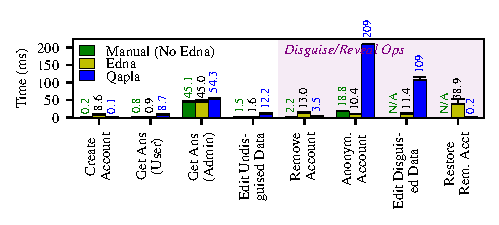
\includegraphics[width=\columnwidth]{figs/websubmit_qapla_op_stats}
    \caption[Latencies of Websubmit operations when implemented with
    Qapla vs. with \sys.]{\sys achieves competitive performance with a manual baseline and
    outperforms Qapla on nearly all common WebSubmit operations (2k users,
    80 answers/user).
    Bars show medians, error bars are 5\textsuperscript{th}/95\textsuperscript{th}
    percentile latencies.}
  \label{f:qapla_ws_opstats}
\end{figure}

%
\subsection{Performance}
\label{s:eval-qapla-perf}
% comparable with \sys.
%
We measure Qapla's performance (Figure~\ref{f:qapla_ws_opstats}) on the 
WebSubmit operations evaluated in \S\ref{s:eval-ops} (Figure~\ref{f:ops-websubmit}).
%
Qapla performs well on operations that require only writes, since Qapla does not
rewrite write queries.  Removing and restoring accounts requires only a single
metadata flag update in Qapla, whereas \sys encrypts/decrypts user data and
actually deletes it from the database.
%
However, Qapla rewrites all read queries, so Qapla performs poorly on operations
that require reads, such as listing answers and editing (disguised or
undisguised) data.
%
Qapla's query rewriting takes $\approx$1ms, and rewrites \fn{SELECT} queries in
ways that affect performance (\eg adding joins to evaluate predicates).
%
Overall, \sys achieves better performance on read operations.

%
%Furthermore, \sys achieves better performance than Qapla on common operations.
